%%%%%%%%%%%%%%%%%%%%%%%%%%%%%%%%%%%%%%%%%%
%% Master file OMEX Metadata Format specification
%%%%%%%%%%%%%%%%%%%%%%%%%%%%%%%%%%%%%%%%%%
\listfiles
\documentclass[pdftex,rgb,dvipsnames,svgnames,hyperref,table]{report}
\usepackage{etoolbox}

\usepackage[a4paper,centering,margin=1in,marginparwidth=0.75in]{geometry}
\usepackage[utf8]{inputenc} % unicode support
\usepackage{shadow}
\usepackage{supertabular}
\usepackage{multirow}
\usepackage{multicol}
\usepackage{enumitem}
\usepackage{lscape}
\usepackage{layout}
\usepackage{array}
\usepackage{fancybox}
\usepackage{xspace}
\usepackage{ifpdf}
\usepackage{etoolbox}

\usepackage{tocvsec2}

% Hyperref, xcolor, graphicx and possibly others have a flag "pdftex"
% that needs to be used if pdflatex is being used.  The following puts
% these inside a conditional for that situation.

\usepackage[pdftex,rgb,dvipsnames,svgnames,hyperref,table]{xcolor}

\usepackage{float}
\usepackage[american]{varioref}
\usepackage[normalem]{ulem}
\usepackage{eso-pic}
\usepackage{natbib}
\usepackage{listings} % enabling listings

\usepackage{url} % enabling URLs

\usepackage{pifont}% enable dingbats
\usepackage{alltt}

% using pdflatex with emp package
 \ifx\pdftexversion\undefined
 \usepackage[dvips]{graphicx}
 \else
 \usepackage[pdftex]{graphicx}
 \graphicspath{{./}{./images/}}
\DeclareGraphicsExtensions{.png}
 \fi

% Hyperref, xcolor, graphicx and possibly others have a flag "pdftex"
% that needs to be used if pdflatex is being used.  The following puts
% these inside a conditional for that situation.

\ifpdf
  % Case: using pdflatex

  \usepackage[pdftex]{graphicx}
  \DeclareGraphicsExtensions{.pdf,.png}

  % Options get even more complicated.  If we're producing grayscale output,
  % we don't want to bother with coloring links, but we still want to load
  % hyperref so that its macros are defined (and we don't have to redefine
  % everything that uses hyperref).  So:

  \usepackage[pdftex,breaklinks=true,colorlinks=true,plainpages=false,
  pdfpagelabels,bookmarks=true,bookmarksopen=true,bookmarksopenlevel=2,
  pdfhighlight=/O,linkcolor={RoyalBlue},citecolor={RoyalBlue},
  urlcolor={RoyalBlue}]{hyperref}

  \usepackage[pdftex,rgb,dvipsnames,svgnames,hyperref,table]{xcolor}

\else
  % Case: not using pdflatex

  \usepackage{graphicx}
  \DeclareGraphicsExtensions{.eps,.png}

  \usepackage[breaklinks,plainpages=false,pdfpagelabels]{hyperref}
  \usepackage[rgb,dvipsnames,svgnames,hyperref,table]{xcolor}

\fi

% Package 'rotating' needs to come after the others.

\usepackage{rotating}

% Booktabs for sharp-looking \toprule, \midrule, \bottomrule in tables.

\usepackage{booktabs}
\setlength{\cmidrulewidth}{0.3 pt}
\setlength{\lightrulewidth}{0.3 pt}
\setlength{\heavyrulewidth}{0.9 pt}
\setlength{\parindent}{0pt} % no indents in the whole document

%% ----------------------------------------------------------------------------
%% Special customizations
%% ----------------------------------------------------------------------------

\makeatletter

% Adjust bottom-of-page behavior and page line spacing.

\raggedbottom
\renewcommand{\baselinestretch}{0.98}

% Numbers the paragraph, but does not lists them in the ToC

\setcounter{secnumdepth}{4}
\setcounter{tocdepth}{2}

% Fix placement of figures & tables.  This keeps latex from shoving big
% floats to the end of a document when they are somewhat big, which it will
% do even if you put [htb] as the argument.

\setcounter{topnumber}{3}
\renewcommand\topfraction{1.0}
\setcounter{bottomnumber}{2}
\renewcommand\bottomfraction{1.0}
\renewcommand\textfraction{0.0}
\renewcommand\floatpagefraction{0.9}

% Adjustment to the spacing around tables and figures.

\renewcommand{\intextsep}{2em}

% This sets up Helvetica for headings.  The font scaling is
% because the default Helvetica size is too big.

\RequirePackage{helvet}
\def\Hv@scale{0.87}

% The following sets up txtt for the typewriter font.

\renewcommand{\ttdefault}{txtt}
\DeclareMathAlphabet{\mathtt}{OT1}{txtt}{m}{n}
\SetMathAlphabet{\mathtt}{bold}{OT1}{txtt}{b}{n}

% The next bit is an adaption of code from ot1phv.fd and adapted to the txtt
% fonts.  The txtt fonts are just a tad too big, so this tries to rescale
% them down a tiny bit.  This isn't completely right because I couldn't
% figure out the right syntax when the DeclareFontShape uses ssub below.
% (Notice how the ones with ssub don't have the \Txtt@@scale factor.)

\def\Txtt@scale{0.975}
\edef\Txtt@@scale{s*[\csname Txtt@scale\endcsname]}%

\DeclareFontFamily{OT1}{txtt}{\hyphenchar \font\m@ne}
\DeclareFontShape{OT1}{txtt}{m}{n}{	%rebular
     <-> \Txtt@@scale txtt%
}{}
\DeclareFontShape{OT1}{txtt}{m}{sc}{	%cap & small cap
     <-> \Txtt@@scale txttsc%
}{}
\DeclareFontShape{OT1}{txtt}{m}{sl}{	%slanted
     <-> \Txtt@@scale txttsl%
}{}
\DeclareFontShape{OT1}{txtt}{m}{it}{	%italic
     <-> ssub * txtt/m/sl%
}{}
\DeclareFontShape{OT1}{txtt}{m}{ui}{	%unslanted italic
     <-> ssub * txtt/m/sl%
}{}
\DeclareFontShape{OT1}{txtt}{b}{n}{	%bold
     <-> \Txtt@@scale txbtt%
}{}
\DeclareFontShape{OT1}{txtt}{b}{sc}{	%bold cap & small cap
     <-> \Txtt@@scale txbttsc%
}{}
\DeclareFontShape{OT1}{txtt}{b}{sl}{	%bold slanted
     <-> \Txtt@@scale txbttsl%
}{}
\DeclareFontShape{OT1}{txtt}{b}{it}{	%bold italic
     <-> ssub * txtt/b/sl%
}{}
\DeclareFontShape{OT1}{txtt}{b}{ui}{	%bold unslanted italic
     <-> ssub * txtt/b/sl%
}{}
\DeclareFontShape{OT1}{txtt}{bx}{n}{	%bold extended
     <-> ssub * txtt/b/n%
}{}
\DeclareFontShape{OT1}{txtt}{bx}{sc}{	%bold extended cap & small cap
     <-> ssub * txtt/b/sc%
}{}
\DeclareFontShape{OT1}{txtt}{bx}{sl}{	%bold extended slanted
     <-> ssub * txtt/b/sl%
}{}
\DeclareFontShape{OT1}{txtt}{bx}{it}{	%bold extended italic
     <-> ssub * txtt/b/sl%
}{}
\DeclareFontShape{OT1}{txtt}{bx}{ui}{	%bold extended unslanted italic
     <-> ssub * txtt/b/sl%
}{}

% This next set of commands uses the sectsty package to change
% section labels to be in a sans-serif font and put the numbers
% into the left margin.

\usepackage{sectsty}
\allsectionsfont{\sffamily\raggedright}
\def\@seccntformat#1{\protect\makebox[0pt][r]{\csname the#1\endcsname\quad}}

% The next definitions change the style of the section headings.

% Definition of paragraph style.

\setlength{\parindent}{0 pt}            % Unindented paragraphs, separated ...
\setlength{\parskip}{1.3 ex}            % ... by roughly one blank line.
\setlength{\partopsep}{-1ex plus 0.1ex minus -0.2ex}
\setlength{\itemsep}{-0.25ex plus 0.15ex}

% \topsep is supposed to affect list environments like itemize,
% but does nothing there.  Instead, it affects environments like tabular.

\setlength{\topsep}{0.3ex plus 0.1ex minus -0.2ex}

% Definition of section heading style.

%\renewcommand{\section}{\newpage\@startsection%
%  {section}{1}{0pt}{-1.8ex \@plus -1ex \@minus -.2ex}%
%  {0.8ex}{\clearpage\normalfont\Large\bfseries\sffamily}}

\renewcommand{\chapter}{\@startsection%
  {chapter}{1}{0pt}{-1.8ex \@plus -1ex \@minus -.2ex}%
  {0.8ex}{\normalfont\Huge\bfseries\sffamily}}
  
\renewcommand{\section}{\@startsection%
  {section}{1}{0pt}{-1.8ex \@plus -1ex \@minus -.2ex}%
  {0.8ex}{\normalfont\Large\bfseries\sffamily}}



\renewcommand{\subsection}{\@startsection%
  {subsection}{2}{0pt}{-2ex \@plus 1ex \@minus -.2ex}%
  {0.8ex}{\large\bfseries\sffamily}}

\renewcommand{\subsubsection}{\@startsection%
  {subsubsection}{3}{0pt}{-1.5ex \@plus 1ex \@minus -.2ex}%
  {0.5ex}{\slshape\normalsize\bfseries\sffamily}}

\renewcommand{\paragraph}{\@startsection%
  {paragraph}{4}{0pt}{-1.25ex \@plus 1ex \@minus -.2ex}%
  {0.5ex}{\slshape\normalsize\sffamily}}


% Below, we take out the heading embedded by the \tableofcontents
% command so that we can control where it's put.

\renewcommand\tableofcontents{%
    \if@twocolumn
      \@restonecoltrue\onecolumn
    \else
      \@restonecolfalse
    \fi
    \@starttoc{toc}%
    \if@restonecol\twocolumn\fi
}

% There seems to be no way to redefine the font used by the table of contents
% line printing command except to modify the source from latex.ltx.

\def\@dottedtocline#1#2#3#4#5{%
  \ifnum #1>\c@tocdepth \else
    \vskip \z@ \@plus.2\p@
    {\leftskip #2\relax \rightskip \@tocrmarg \parfillskip -\rightskip
     \parindent #2\relax\@afterindenttrue
     \interlinepenalty\@M
     \leavevmode
     \@tempdima #3\relax
     \advance\leftskip \@tempdima \null\nobreak\hskip -\leftskip
     {#4}\nobreak
     \leaders\hbox{$\m@th
        \mkern \@dotsep mu\hbox{.}\mkern \@dotsep
        mu$}\hfill
     \nobreak
     \hb@xt@\@pnumwidth{\hfil\normalfont\sffamily \normalcolor #5}%
     \par}%
  \fi}

% The following was ripped out of caption.sty, version 1.4b.
% Copyright (C) 1994-95 Harald Axel Sommerfeldt
% The first few lines set up the parameters for the layout created
% by this style file.

\newcommand{\captionsize}{\small}
\newcommand{\captionfont}{\captionsize\itshape}
\newcommand{\captionlabelfont}{\captionsize\sffamily\bfseries\upshape}
\newlength{\captionmargin}
\setlength{\captionmargin}{6ex}

\newsavebox{\as@captionbox}
\newlength{\as@captionwidth}
\newcommand{\as@normalcaption}[2]{%
  #1 #2\par}
\let\as@caption\as@normalcaption
\newcommand{\as@centercaption}[2]{%
  \parbox[t]{\as@captionwidth}{{\centering#1 #2\par}}}
\let\as@shortcaption\as@centercaption
\newcommand{\as@makecaption}[2]{%
  \setlength{\leftskip}{\captionmargin}%
  \setlength{\rightskip}{\captionmargin}%
  \addtolength{\as@captionwidth}{-2\captionmargin}%
  \renewcommand{\baselinestretch}{0.9}
  \captionfont%
  \sbox{\as@captionbox}{{\captionlabelfont #1:} #2}%
  \ifdim \wd\as@captionbox >\as@captionwidth
    \as@caption{{\captionlabelfont #1:}}{#2}%
  \else%
    \as@shortcaption{{\captionlabelfont #1:}}{#2}%
  \fi}
\renewcommand{\@makecaption}[2]{%
  \vskip\abovecaptionskip%
  \setlength{\as@captionwidth}{\linewidth}%
  \as@makecaption{#1}{#2}%
  \vskip\belowcaptionskip}
\ifx\@makerotcaption\undefined
\else
  \typeout{\space\space\space\space\space\space\space\space\space
           `rotating' package detected}
  \renewcommand{\@makerotcaption}[2]{%
    \renewcommand{\baselinestretch}{0.9}
    \captionfont%
    \sbox{\as@captionbox}{{\captionlabelfont #1:} #2}%
    \ifdim \wd\as@captionbox > .8\vsize
      \rotatebox{90}{%
        \setlength{\as@captionwidth}{.8\textheight}%
        \begin{minipage}{\as@captionwidth}%
          \as@caption{{\captionlabelfont #1:}}{#2}%
        \end{minipage}}\par
    \else%
      \rotatebox{90}{\usebox{\as@captionbox}}%
    \fi
    \hspace{12pt}}
\fi
\ifx\floatc@plain\undefined
\else
  \typeout{\space\space\space\space\space\space\space\space\space
           `float' package detected}
  \renewcommand\floatc@plain[2]{%
    \setlength{\as@captionwidth}{\linewidth}%
    \as@makecaption{#1}{#2}}
  \ifx\as@ruled\undefined
  \else
    \renewcommand\floatc@ruled[2]{%
      \setlength{\as@captionwidth}{\linewidth}%
      \renewcommand{\baselinestretch}{0.9}
      \captionfont%
      \as@caption{{\captionlabelfont #1:}}{#2}}
  \fi
\fi

\renewcommand{\@makechapterhead}[1]{%
\vspace*{50 pt}%
{\setlength{\parindent}{0pt} \raggedright% \normalfont
\sffamily\bfseries\Huge\thechapter.\ #1
\par\nobreak\vspace{40 pt}}}

\makeatother

% packages and commands
%%%%%%%%%%%%%%%%%%%%%%%%%%%%%%%%%%%%%%%%%%%%%%%%%%%%%%%%%%%%%%%%%%
%%  Commands
%%%%%%%%%%%%%%%%%%%%%%%%%%%%%%%%%%%%%%%%%%%%%%%%%%%%%%%%%%%%%%%%%%

\newcommand{\code}[1]{\texttt{#1}}
\newcommand{\token}[1]{\texttt{#1}}
\newcommand{\concept}[1]{\textcolor{blue}{#1}}
\newcommand{\element}[1]{\texttt{#1}}
\newcommand{\alert}[1]{\textcolor{red}{#1}}
\newcommand{\note}[1]{\paragraph*{} \emph{\scshape{\alert{Please Note}}: #1} \newline}
\newcommand{\mailto}[1]   {\link{mailto:#1}{#1}}
\newcommand{\link}[2]     {\literalFont{\href{#1}{#2}}}
\newcommand{\literalFont}[1]{\textup{\texttt{#1}}}
\newcommand{\version}{2\xspace}
\newcommand{\level}{1\xspace}
\newcommand{\LoneVone}{Level~1 Version~1\xspace}
\newcommand{\LoneVtwo}{Level~1 Version~2\xspace}
\newcommand{\LoneVthree}{Level~1 Version~3\xspace}
\newcommand{\currentLV}{Level~1 Version~1\xspace}
\newcommand{\previousLV}{Level~1 Version~2\xspace}
\newcommand{\biom}{BioModels Database\xspace}
% attribute table layout
\newcommand{\attribute}{attribute\xspace}
\newcommand{\desc}{description\xspace}
\newcommand{\subelements}{sub-elements\xspace}

\newcommand{\SedModel}{\hyperref[class:model]{Model}\xspace}
\newcommand{\SedDataSource}{\hyperref[class:dataSource]{DataSource}\xspace}
\newcommand{\SedDataDescription}{\hyperref[class:dataDescription]{DataDescription}\xspace}
\newcommand{\SedSlice}{\hyperref[class:slice]{Slice}\xspace}

\newcommand{\refpage}[1]{\hyperref[#1]{page \pageref{#1}}} % to hyperref to a particular page in the spec
\newcommand{\tabcap}[1]{  % to create table captions for overview tables for each SED-ML class
Attributes and nested elements for \concept{#1}. \emph{xy$^{o}$} denotes optional elements and attributes.
}

\newcommand{\tabtext}[2]{ % to create the introducing table text for each table reference
\tab{#1}~shows all attributes and sub-elements for the \concept{#2} element as defined by the SED-ML \currentLV XML Schema.
}

\newcommand{\lsttext}[2]{ % to create the introducing listing text for each listing reference
  Listing~\vref{lst:#1} shows the use of the \element{#2} element in a SED-ML file as defined by the SED-ML \currentLV XML Schema.
}

\newcommand{\lsttexta}[2]{ % to create the introducing listing text for each listing reference
  Listing~\vref{lst:#1} shows the use of the \element{#2} attribute in a SED-ML file as defined by the SED-ML \currentLV XML Schema.
}

%
\newcommand{\chap}[1]     {Chapter~\protect\ref{chap:#1}\xspace}
\newcommand{\sect}[1]     {Section~\protect\ref{sec:#1}\xspace}
\newcommand{\fig}[1]      {Figure~\protect\vref{fig:#1}\xspace}
\newcommand{\tab}[1]      {Table~\protect\vref{tab:#1}\xspace}
\newcommand{\lst}[1]      {Listing~\protect\ref{lst:#1}\xspace}
\newcommand{\eg}          {e.\,g.,\xspace}
\newcommand{\ie}          {i.\,e.,\xspace}

\newcommand{\tickYes}{\hspace{1pt}\ding{52}}
\newcommand{\tickNo}{\hspace{1pt}\ding{56}}


%%%%%%%%%%%%%%%%%%%%%%%%%%%%%%%%%%%%%%%%%%%%%%%%%%%%%%%%%%%%%%%%%%
%%  environments
%%%%%%%%%%%%%%%%%%%%%%%%%%%%%%%%%%%%%%%%%%%%%%%%%%%%%%%%%%%%%%%%%%

% standard figure layout
\newcommand{\sedfig}[4][]
% 	 {\begin{figure}[H]\begin{center}{\includegraphics[width=0.9\textwidth,#1]{#2}}\caption{#3}\label{#4}\end{center}\end{figure}}
	 {\begin{figure}[hbt!]\begin{center}{\includegraphics[width=0.9\textwidth,#1]{#2}}\caption{#3}\label{#4}\end{center}\end{figure}}

\newcommand{\sedfigX}[4][]
	{\begin{figure}[H]\begin{center}{\includegraphics[#1]{#2}}\caption{#3}\label{#4}\end{center}\end{figure}}

% standard XML listing layout
\lstnewenvironment{myXmlLst}[2]
	{\lstset{basicstyle=\ttfamily\scriptsize, caption={#1},label={#2}, keywordstyle=\color{blue}\bfseries, stringstyle=\color{blue}, commentstyle=\color{red}, captionpos=b, breaklines=true, xleftmargin=1.5em, xrightmargin=1.5em, numbers=left, numberstyle=\ttfamily\tiny, numbersep=5pt, tabsize=4, showstringspaces=false, language=XML}} %, float=!h
	{}

% listings in appendixes:
\newcommand{\myXmlImport}[3]	{\lstinputlisting[basicstyle=\ttfamily\scriptsize,caption={#1},label={#2},%
	keywordstyle=\color{blue}\bfseries, stringstyle=\color{blue}, commentstyle=\color{red}, captionpos=b, breaklines=true, xleftmargin=1.5em, xrightmargin=1.5em, numbers=left, numberstyle=\ttfamily\tiny, numbersep=5pt, tabsize=4, showstringspaces=false, language=XML, stepnumber=1]{#3}} %float=h!

%% Conditional for L1V4 updates
\newbool{L1V4}
\setbool{L1V4}{true}

% END \input{sources/latex-macros.tex}




\begin{document}
\begin{titlepage}


\begin{center}

\textbf{\sffamily\bfseries\huge
OMEX Metadata Specification version 1.1\\[0.3em]
}

\vspace*{0.75in}

\large
\today\\[0.25in]

% \cornersize{0.3}\ovalbox{\begin{minipage}{4.9in}\color{DarkRed}
% Disclaimer: This is a working draft of the OMEX Metadata standard. 
% It is not a normative document.
% \end{minipage}}

\vspace{0.5in}

{\bf Lead Developer:} Maxwell Neal
\paragraph*{}
\textbf{\sffamily Editors}\\[7pt]
\begin{tabular}{l>{\hspace*{15pt}}r}
John Gennari & \emph{University of Washington} \\
Dagmar Waltemath & \emph{Universitätsmedizin Greifswald} \\
David Nickerson & \emph{University of Auckland}\\
Matthias K\"onig& \emph{Humboldt-Universität zu Berlin}\\
\end{tabular}

% Feedback included in this document:
% - Nick Juty

\vspace{1.2in}

\normalsize
\begin{minipage}{5in}
\begin{center}
  The latest release of the specification is available at: \url{https://co.mbine.org/specifications/omex-metadata}
  \paragraph*{}
  To discuss any aspect of the current specification as well as language details, please post a message 
    to the COMBINE annotation forum:
    \url{https://groups.google.com/forum/#!forum/combine-annot}
  \paragraph*{}
%  To get subscribed to the mailing list, please write to the same address \mailto{omexmetadata@abc.net}.
%  \paragraph*{}
%  To contact the authors of the OMEX Metadata specification, please write to \mailto{omexmetadata-editors@abc.net}
\end{center}
\end{minipage}
\vfill


\end{center}

\end{titlepage}

\setcounter{page}{2}
\textbf{\sffamily\bfseries\huge   }
\vspace{0.2in}

\textbf{\sffamily\bfseries\huge
Contents
}
\vspace{0.2in}

\tableofcontents

\newpage



% ~~~~~~~~~~~~~~~~~~~~~~~~~~~~~~~~~~~~~~~~
%% INTRODUCTION
% ~~~~~~~~~~~~~~~~~~~~~~~~~~~~~~~~~~~~~~~~
\chapter{Introduction}
\vspace{5mm}

\section{Motivation}
Metadata annotations enhance the interoperability, reusability, comparability, and comprehension of computational biological models. Annotations can capture the biological meaning of what a model simulates, specify precisely the components comprising a model, describe a model's provenance, provide layout information for visualizing a model's architecture, etc. These annotations can be leveraged to make it easier for researchers to find and re-purpose models, re-combine models and model parts, and integrate models across repositories and experimental data stores. For example, semantic annotations can be leveraged to enhance model search capabilities by identifying models that overlap in terms of the biological phenomena they represent. 

Realizing the potential benefits of annotation requires the development of standards that adhere to a community-based annotation protocol. Without such standards, researchers must account for a variety of annotation formats and approaches, a situation that can become prohibitively cumbersome and which can defeat the purpose of annotating a model.

This document was created to specify how to represent model annotations within the Open Modeling and EXchange (OMEX) file format \cite{Bergmann2014}. Our goal is to harmonize and simplify the representation of metadata annotations in models that are shared among the biological research community regardless of the models' encoding format. Our hope is that community-wide adherence to this specification will significantly advance the community's ability to discover relevant models and data sets as well as to re-purpose/re-combine models and model components. 

\label{motivation:example}
\subsection{Cross-format search}
Researchers cannot easily search across model repositories for models that simulate a particular biological process. As illustrated by Henkel, et al. \cite{Henkel2015}, if the annotations on models in various repositories were encoded according to a common standard, this would make it easier to develop tools for searching across repositories and modeling formats.

\subsection{Semantic similarity between models}
Using standardized metadata annotations to capture the biological properties simulated by a model allows developers to quantify how similar two models are in terms of the biological phenomena they represent (see, for example, \cite{Schulz2011,Henkel2018}). Such objective measures of biological similarity are critical for developing tools that help users discover related models within and across model repositories, exposing users to new models that may be relevant to their research.

\subsection{Semantics-based composition}
Thorough semantic annotations on models are also critical for performing semantics-based model composition. This compositional approach, which aims to reduce the time and code-level edits required to merge models into larger systems, leverages machine-readable semantic annotations to automatically propose biologically-consistent interfaces between models \cite{Neal2014}. The use of a consistent annotation protocol is necessary for achieving this level of composability for biological models.

\subsection{Semantic integration of empirical data and simulation models}
Given that models are largely intended to reproduce, explain, and predict empirical data measurements, any general solution for annotating model elements would also be applicable for annotating empirical data used for model parameterization and validation. For example, the same semantic annotation on a CellML model variable that represents aortic blood pressure could be used to annotate an empirical aortic blood pressure measurement recorded in a data file. Using a common, standardized approach for annotating models as well as empirical data would accelerate the development of tools that help modelers discover data sets of interest for model parameterization or validation and help experimentalists discover models of interest for use in analyses. 


 \label{sec:intro1}
\pagebreak

% ~~~~~~~~~~~~~~~~~~~~~~~~~~~~~~~~~~~~~~~~
%% TECHNICAL SPECIFICATION
% ~~~~~~~~~~~~~~~~~~~~~~~~~~~~~~~~~~~~~~~~
\chapter{OMEX Metadata technical specification}
\vspace{5mm}

\label{chp:specification}
This section presents the technical specification for associating metadata with the contents of COMBINE archives \cite{Bergmann2014} in the OMEX file format.

%% NOTATION CONVENTIONS
\section{Conventions used in this document}
Resource Description Framework (RDF, \url{https://www.w3.org/RDF/}) content and in-paragraph references to RDF subjects, predicates, and objects are 
1
 indicated by \texttt{typewriter font}.

The table below indicates the prefixes used in RDF Uniform Resource Identifiers (URIs) and their namespaces.
\begin{center}
 \begin{tabular}{||c c||} 
 \hline
 Prefix & Namespace \\
 \hline\hline
 rdf & http://www.w3.org/1999/02/22-rdf-syntax-ns\# \\ 
 \hline
 dcterms & http://purl.org/dc/terms/ \\
 \hline
 bqbiol & http://biomodels.net/biology-qualifiers/ \\
 \hline
 bqmodel & http://biomodels.net/model-qualifiers/ \\
 \hline
 semsim & http://www.bhi.washington.edu/semsim\# \\
 \hline
\end{tabular}
\end{center}

\label{sec:conventions}

%% CONCEPTS
\section{Concepts used in OMEX Metadata}
\subsection{COMBINE archives}
A COMBINE archive (also known as an OMEX archive) is a single file containing the various documents necessary for the description of a model as well as all associated data and simulation procedures. These documents include, for example, simulation experiment descriptions, all models needed to run the simulations, associated data files, etc. The archive is encoded using the OMEX format. Version 1 of the OMEX specification is available at \url{https://co.mbine.org/freelinking/standards/omex/version-1}.

\subsection{RDF}
The Resource Description Framework (RDF) is a World Wide Web Consortium-recommended standard for representing information on the Web. RDF consists of statements built using subject-predicate-object triples that can be used to assert relationships between model components and terms from online knowledge resources. A primer on RDF is available at \url{https://www.w3.org/TR/rdf11-concepts/}, and links to examples of RDF-encoded model annotations can be found in this document.

\subsection{Model-level annotations}
A model-level annotation is an annotation that captures an aspect of the model \textit{as a whole}. Examples include an annotation that indicates the PubMed ID of the model's source publication, an annotation that indicates that the model simulates glycolysis, or an annotation that indicates the identity of the curator who encoded the model. 

\subsection{Archive-level annotations}
Archive-level annotations are metadata items that capture information about the archive as a whole. These may be especially important when the archive includes multiple models. These annotations can also be used to explain relationship across multiple files -- e.g., how or why a sed.ml file captures a particular simulation result from the model.

\subsection{Model component annotations}
A model component annotation is a computer-accessible metadata item that captures, entirely or in part, the meaning of a model component or data element. For example, an annotation on a model variable might indicate that it represents the concentration of cytosolic glucose in a pancreatic beta cell or it might describe a purely computational feature such as the simulation time step.

\subsection{Singular annotations}
Singular annotations are those that are comprised of a single RDF statement linking a model or data element to a knowledge resource term. These are the types of annotations currently found throughout curated models on \href{http://www.ebi.ac.uk/biomodels/}{BioModels}. See section \ref{singularanns} for examples.

\subsection{Composite annotations}
Composite annotations are semantic annotations that are comprised of multiple annotation terms linked using standard qualifiers (also known as ``relations" or ``predicates") to indicate the precise biological meaning of a model or data element. Composite annotations are used when a single knowledge resource term is not available to define a model or data element. Composite annotations have two primary components: the physical property represented by the annotated item (e.g., chemical concentration, fluid volume) and the physical entity, process, force, or dependency that bears the property (e.g., a pool of ATP, blood in a cardiac cavity, the glucokinase reaction). See section \ref{CSAs} for examples.

\subsection{identifiers.org URIs}
identifiers.org \cite{identifiers2018} is a resolving system that enables referencing of data for the scientific community with a focus on the life sciences domain. It handles persistent identifiers in the form of URIs and Compact URIs (CURIEs). identifiers.org also provides standardized URI prefixes for a large set of biological knowledge resources.

\subsection{BioModels.net qualifiers}
BioModels.net qualifiers are a set of standardized relations (also known as ``predicates") used to indicate the nature of the relationship articulated in an annotation, or in an annotation component. For example, the BioModels.net qualifier \texttt{is} is used to indicate the identity of an annotated element and the qualifier \texttt{isEncodedBy} is used to indicate that a particular protein is encoded by a particular DNA sequence.

\subsection{Metadata identifiers}
In standardized XML-based model exchange formats such as the Systems Biology Markup Language (SBML \cite{SBML2003}), CellML \cite{CellML2003}, NeuroML \cite{NeuroML} and the Simulation Experiment Description Markup Language (SED-ML \cite{SEDML}), the XML elements often have an attribute for specifying a metadata identifier (ID). For example, the following SBML code from model BIOMD0000000001 on BioModels.net indicates that the model has metadata ID ``\_000001".

\verb|     <model metaid="_000001" id="BIOMD0000000001" name="Edelstein1996 - EPSP ACh event">|\\*
\verb|     ...|\\*
\verb|     </model>|\\*

These metadata IDs are unique to each XML element and are used in annotation statements to link annotations to the XML elements in a COMBINE archive that they describe.
  
\section{Serializing OMEX Metadata}
The specification for serializing annotations in OMEX-formatted documents is based largely on the article by Neal et al. \cite{Neal2019}, which presents a list of recommendations for standardizing semantic annotations on biological models. This part of the specification addresses how to standardize the storage of annotations within COMBINE archives, an essential technical prerequisite for harmonizing their representation across model annotation efforts.

\subsection{Serialization format}
We recommend encoding OMEX metadata in RDF. RDF has emerged as the \textit{de facto} standard for encoding annotations among the COMBINE community, and all COMBINE standards currently use it. Although more expressive knowledge representation formats exist, RDF is sufficiently expressive for articulating the kinds of annotations required to catalyze significant advances in model discovery, reuse and integration. We recommend RDF content be formatted as RDF/XML as this is the format most widely supported by software libraries. However, annotations can be formatted as Turtle (\href{https://www.w3.org/TR/turtle/}{https://www.w3.org/TR/turtle/}) or $n$-triples (\url{https://www.w3.org/TR/n-triples/}) as well. Software that supports reading/writing COMBINE archive annotation files should support these alternative formats in addition to RDF/XML.

\subsection{Separation of annotations from models and data}
We recommend using separate RDF files to store all annotations associated with model and simulation protocol files within a COMBINE archive. The traditional practice within the COMBINE community has been to serialize annotations within the same file that specifies the model’s computational aspects. There are several reasons why we recommend storing semantic annotations in a separate file, instead. First, this will normalize the format in which annotations are stored across the different COMBINE standards. Currently, the exact format used to store annotations within model files differs among standards. Normalizing the format will simplify the development of software that provides programmatic manipulation of annotations. It will also allow for better separation between modeling and annotation tasks, removing the burden of supporting annotation from the software teams that are developing software libraries for specific COMBINE standards.

We also recommend storing annotation files separately because we recognize that different research groups may have different preferences for which knowledge resources to use for annotation. Externalizing annotations in a separate file allows a single model file to be referenced by multiple annotation files, allowing different research groups to describe the same modeling resource in different ways. This approach follows the vision of the COMBINE archive, wherein multiple types of modeling files are archived together to make simulation experiments readily reproducible and shareable among research groups. When sharing models, we recommend that annotations be distributed along with the files they annotate, and COMBINE archives provide a standardized way to bundle such files together. An additional advantage of storing annotations in a separate file is that the RDF content can be serialized in various formats, including XML or Turtle. Currently, the serialization is dictated by the model format.

Storing annotations in a separate file requires keeping them synchronized. For example, if a variable identifier changes in the model file, that change should be reflected in the annotation file(s) as well. We recommend that the community encourages the development of software libraries and tools that help ensure coordination between a model’s computational aspects and its annotations.

Multiple RDF annotation files are allowed within an archive and the OMEX manifest file should provide sufficient information so that parsers can automatically determine which files within an archive contain the RDF annotations. Software tools should provide support for reading the content of each individual annotation file into separate RDF graphs and, alternatively, for reading the content of multiple files into one merged RDF graph.


\subsection{Formatting URIs in RDF}
The subjects of RDF triples used for annotation should be relative URIs, giving the name of the file to be annotated, and the metadata ID of the annotated element within the file as the URI fragment. To emphasize that the URI is local to the archive it may be prepended with "./", although this is not required. For example, if there is a model file in a COMBINE archive named MyModel.xml, and it contains an element with metadata ID ``meta0", then the subject URI used in an annotation statement on that model element would be:

\verb|  ./MyModel.xml#meta0|

Wherever possible, COMBINE archive annotation documents should use BioModels.net qualifiers in RDF statements that define model elements. These existing qualifiers provide a basic level of coverage needed for articulating annotations in models, and they are specifically intended for use in statements that link computational abstractions of physical phenomena to knowledge resource terms representing the material manifestations of those phenomena. 

In addition to BioModels.net qualifiers to encode singular annotations, SemSim qualifiers should be used in composite annotations to unambiguously encode the relationships between the annotation's components (see \ref{CSAs}). As illustrated in the examples in \ref{CSAs}, SemSim qualifiers are primarily used to indicate physical entity participation in a physical process or physical force as well as the stoichiometry of a process's participants.

We recommend using the identifiers.org URI format when referencing knowledge resource terms in RDF statements: identifiers.org supports a vast set of biological knowledge resources used for annotation and identifiers.org-formatted URIs are resolvable. The identifiers.org services are also capable of more complex URI resolution compared to alternative services. For example, identifiers.org is specifically built to address downtime and changing endpoints and directs users to an alternative site for a given data record as long as one is listed (one-to-many mappings) whereas persistent uniform resource locator services specify only one endpoint for URI resolution (one-to-one mappings). We also recommend using identifiers.org-formatted URIs because they use a simple, uniform nested structure that facilitates generation and parsing, and because identifiers.org reuses data providers’ record identifiers.

\subsection{Serializing model-level annotations}
\textcolor{magenta} {New text goes here....\\
Hmmm. what's the name space for any of my new model-level annotations?}

\begin{itemize}
    \item \emph {model-author} This refers to the contact author of the model. This is usually the lead or contact author for the associated publication. This author may be different (of course) from the archive author or the model curator. 
    \item \emph{model-curator} If available, this is the name of the person who provided the annotations for this model. This may be the same as the model-author. 
    \item \emph{isDescribedBy} This is a pointer to the publication for the model. For example, a pubMed ID, or some other unique ID.
    \item \emph{model-taxon} If applicable, this annotation describes the biological entity (e.g. species) to which the model applies. This may also be the biological entity from which the data was collected that was used to build the model. This annotation should point to something like the NCBI Taxonomy resource. 
\end{itemize}

The following is an example of a singular, model-level, annotation that indicates the PubMed ID of the model's source publication. In this case, the metadata ID for the model as a whole (e.g., the metadata ID associated with the $<$model$>$ element in an SBML model) is ``modelmeta1". (The rdf syntax used here and throughout the document is Turtle.) 
 
 \verb| @prefix bqmodel: <http://biomodels.net/model-qualifiers/> . |\\*
 \verb| @prefix pubmed: <https:identifiers.org/pubmed/> . |\\*
 
 \verb| <./MyModel.sbml#modelmeta1> bqmodel:isDescribedBy pubmed:12991237> . |\\*
 
.... such as those that describe model curation, provenance (including nanopublications), confidence levels, or layout information for model visualization tools. 

We also note that there is currently a proposal to use ORCID identifiers rather than VCard-formatted RDF blocks for indicating the identities of people in these types of annotations. We encourage further debate on this issue within the community.  

\subsection{Serializing archive-level annotations}
\textcolor{magenta} {New text goes here....\\
hmmm}


\subsection{Serializing model component singular annotations}
\label{singularanns}
Singular annotations within COMBINE archive annotation files should be encoded as a single RDF triple. The subject of the triple is the annotated element and should be formatted as a relative URI. The predicate is the URI of a BioModels.net qualifier linking the subject to a URI from a knowledge resource or the Dublin Core Metadata Terms (\url{https://dublincore.org/specifications/dublin-core/dcmi-terms/}) qualifier \texttt{description}. The object of the triple should be an identifiers.org-formatted URI indicating a concept in a knowledge resource, or a text string for free-text definitions of model elements.

 
The following is an example singular semantic annotation indicating that the model element with metadata ID ``meta1" from the model file ``MyModel.xml" represents adenosine tri-phosphate:

 \verb|     <rdf:Description rdf:about="./MyModel.xml#meta1">|\\*
 \verb|      <bqbiol:is rdf:resource="https://identifiers.org/chebi/CHEBI:15422" />|\\*
 \verb|     </rdf:Description>|\\*

The following is an example free-text description of a model variable with metadata ID ``meta2": 

 \verb|     <rdf:Description rdf:about="./MyModel.xml#meta2">|\\*
 \verb|      <dcterms:description>Cardiomyocyte cytosolic ATP concentration</dcterms:description>|\\*
 \verb|     </rdf:Description>|\\*
 

\subsection{Serializing model-component composite annotations} \label{CSAs}
Composite semantic annotations (CSAs) are used to capture the biological meaning of model or data elements when no singular reference term is available that provides a precise enough definition. Based on the SemSim framework \cite{Gennari2011}, CSAs are comprised of two components: the \textit{physical property} that is represented, and what it is a property \textit{of}. The second component, the bearer of the property, is either a physical entity, process, force or dependency. 

\subsubsection{Composite annotation for a property of a physical entity}
\label{CSAentity}

Consider a CellML variable that simulates blood volume in the left coronary artery. The physical property simulated is volume; more precisely, \textit{fluid} volume. This fluid volume is a property of blood in the lumen of the left coronary artery. Because there is no existing knowledge resource term that represents ``blood volume in the left coronary artery", we instead construct a CSA using a combination of existing knowledge resource terms. For the physical property components of CSAs, we recommend using terms from the Ontology of Physics for Biology (OPB \cite{OPB}) because the OPB provides a comprehensive, formally-structured hierarchy of physical properties. In this case, we would use the OPB term ``Fluid volume" (OPB:OPB\_00154). The second part of the CSA (blood in the left ventricle) can be created by linking two terms from the Foundational Model of Anatomy (FMA \cite{FMA}), namely ``Portion of blood" (FMA:9670) and ``Lumen of left coronary artery" (FMA:18228). We link these two FMA terms using the \texttt{isPartOf} BioModels.net qualifier to produce a composite physical entity. The additional statements required in a CSA link the model element being annotated to the physical property it represents (via the \texttt{isVersionOf} BioModels.net qualifier) as well as to the composite physical entity that bears the property (via the \texttt{isPropertyOf} BioModels.net qualifier).

Encoded in RDF/XML, this CSA example would be serialized as:

  \verb|  <rdf:Description rdf:about="./MyModel.xml#VLV">|\\*
  \verb|    <bqbiol:isVersionOf rdf:resource="https://identifiers.org/opb/OPB_00154" />|\\*
  \verb|    <bqbiol:isPropertyOf rdf:resource="#entity_0"/>|\\*
  \verb|  </rdf:Description>|\\*

  \verb|  <rdf:Description rdf:about="#entity_0">|\\*
  \verb|    <bqbiol:is rdf:resource="https://identifiers.org/fma/FMA:9670" />|\\*
  \verb|    <bqbiol:isPartOf rdf:resource="https://identifiers.org/fma/FMA:18228"/>|\\*
  \verb|  </rdf:Description>|\\*

Figure 1 shows a node and edge diagram for the example CSA:
\vspace{5mm}

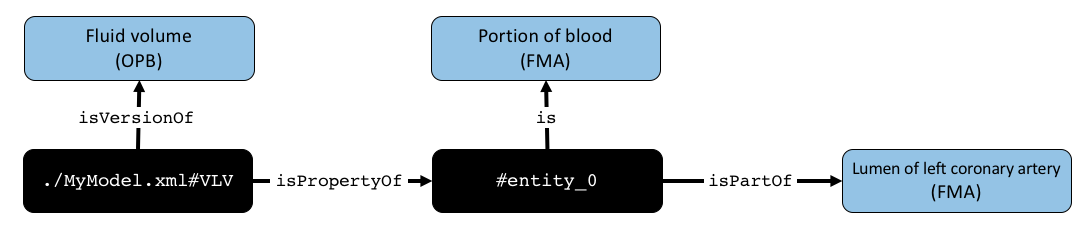
\includegraphics[width=\textwidth]{CSAexample.png}
   \footnotesize Figure 1. Node and edge representation of an example composite annotation for a model variable that simulates blood volume in the left coronary artery. RDF resources local to the OMEX metadata file are in black boxes, external knowledge resource terms are in blue boxes.
\vspace{5mm}

\normalsize
Note that the generic RDF resource \texttt{entity\_0} needs to be created when encoding the CSA. This is required because there are no structures in the CellML schema that represent physical entities, so they are instantiated as RDF resources in the OMEX metadata document. Such instantiation is often not needed for SBML models, since SBML provides explicit XML elements for representing the bearers of physical properties including chemical species, compartments and reactions, and these elements can have unique metadata identifiers assigned to them. 

However, instantiation of a resource that represents the full concept described by the CSA \textit{is} needed for the properties of species, compartments, and reactions in SBML models. While SBML uses XML structures for declaring physical entities ($<$compartment$>$ and $<$species$>$ elements) as well as processes ($<$reaction$>$ elements), it does not declare XML elements that represent the \textit{properties} of those entities and processes. Instead, the property is indicated by an XML attribute on the entities and processes. Therefore, to ensure that these properties are searchable in OMEX annotations, we recommend instantiating a generic RDF resource for each physical property that is implicitly represented in an SBML model. Note that this does not have to be done when annotating an SBML parameter with a CSA because the SBML parameter element includes a metadata ID that can be explicitly referenced in the OMEX metadata file.

\subsubsection{Composite annotation for a property of a physical process}

The example semantic annotation above is for a physical property of a physical entity, however, the physical properties simulated in models or measured experimentally can also be those of physical processes such as chemical reactions, transport of solutes, flow of fluids in vessels, etc. For CSAs on process properties, we recommend the approach created by the developers of the SemSim architecture wherein a custom physical process is instantiated and linked to its energetic sources and sinks as well as mediators whose amounts modulate the magnitude of the physical process property. 

Sources, sinks and mediators are the physical entities that participate in the process: source amounts are consumed by the process, sink amounts are produced, and mediator amounts remain unchanged. Below, we provide  an example of a CSA for the rate of a chemical reaction with one source, one sink, and one mediator. 

First, we assert statements indicating that the model represents a physical property of a process that is a chemical flow rate (OPB:OPB\_00592).

  \verb|  <rdf:Description rdf:about="./MyModel.xml#property_metaid_0">|\\*
  \verb|    <bqbiol:isPropertyOf rdf:resource="./MyModel.xml#process_metaid_0"/>|\\*
  \verb|    <bqbiol:isVersionOf rdf:resource="https://identifiers.org/opb/OPB_00592"/>|\\*
  \verb|  </rdf:Description>|\\*

If this annotation was on a CellML model containing a variable representing the chemical flow rate, the fragment \texttt{property\_metaid\_0} should point to the CellML variable with that metadata ID. If this annotation was on an SBML model that represents the flow rate using a $<$reaction$>$ element and associated attributes, then \texttt{property\_metaid\_0} should be a physical property resource instantiated within the RDF content. The reason is that asserting chemical flow rates via the SBML $<$reaction$>$ structure does not include the explicit construction of an XML element representing the flow rate that can be referenced in the OMEX metadata RDF.

We next assert statements that indicate the physical entity participants in the process: the energetic sources, sinks, and mediators. In this case, there is one source, one sink, and one mediator. The sources and sinks can include stoichiometry statements (using the \texttt{semsim:hasMultiplier} qualifier) to indicate the production/consumption ratios for the process participants (mediator participation statements do not include stoichiometries).

\verb|  <rdf:Description rdf:about="./MyModel.xml#process_metaid_0">|\\*
\verb|    <semsim:hasSourceParticipant rdf:resource="./MyModel.xml#source_0"/>|\\*
\verb|    <semsim:hasSinkParticipant rdf:resource="./MyModel.xml#sink_0"/>|\\*
\verb|    <semsim:hasMediatorParticipant rdf:resource="./MyModel.xml#mediator_0"/>|\\*
\verb|  </rdf:Description>|\\*


\verb|  <rdf:Description rdf:about="./MyModel.xml#source_0">|\\*
\verb|    <semsim:hasMultiplier>1.0</semsim:hasMultiplier>|\\*
\verb|    <semsim:hasPhysicalEntityReference rdf:resource="./MyModel.xml#species_metaid_0"/>|\\*
\verb|  </rdf:Description>|\\*


\verb|  <rdf:Description rdf:about="./MyModel.xml#sink_0">|\\*
\verb|    <semsim:hasMultiplier>2.0</semsim:hasMultiplier>|\\*
\verb|    <semsim:hasPhysicalEntityReference rdf:resource="./MyModel.xml#species_metaid_1"/>|\\*
\verb|  </rdf:Description>|\\*
  
  
\verb|  <rdf:Description rdf:about="./MyModel.xml#mediator_0">|\\*
\verb|    <semsim:hasPhysicalEntityReference rdf:resource="./MyModel.xml#species_metaid_2"/>|\\*
\verb|  </rdf:Description>|\\*
  
RDF statements indicating the biological identity of the chemical species that participate in the process (the resources with the \texttt{species\_metaid\_*} URI fragments in this example) would be included elsewhere in the RDF. For SBML models where these chemical species are explicitly represented using $<$species$>$ elements, the metadata IDs should point to those elements in the SBML code. For other formats, such as CellML, that do not support such elements, the metadata IDs should point to physical entities instantiated elsewhere in the RDF.

We recognize that creating CSAs for biological processes in this manner can duplicate information that is present in an SBML model's reaction network structure. However, we have decided that CSAs for physical processes should be written out in accordance with these guidelines so that all biological features represented in a model are exposed in the RDF metadata alone. This way, the community can more easily apply RDF-processing tools to analyze, query, and reason over semantic metadata in COMBINE archives.  
  
\subsubsection{Composite annotation for a property of a physical force}
CSAs can also be used to represent the properties of physical forces. These include, for example, membrane potentials, chemical potentials and fluid pressures. The structure of CSAs on force properties is similar to process properties. Because forces themselves are not conventionally named or represented explicitly in model code, a force is instantiated as a local resource in the RDF with its energetic sources and sinks specified. (Mediators are only used for process property annotations and stoichiometries are undefined for force participation statements.)

The following is an example CSA that represents the electrical potential caused by a difference in the amount of charged ions on either side of a cell membrane. For this example, we assume a model element with metadata ID ``parameter\_metaid\_0" represents this biological property. 

We assert the triples stating that the model element represents a property of a force, and that it represents the electrical potential (OPB:OPB\_01058) of that force:

  \verb|  <rdf:Description rdf:about="./MyModel.sbml#parameter_metaid_0">|\\*
  \verb|    <bqbiol:isPropertyOf rdf:resource="./MyModel.sbml#force_0"/>|\\*
  \verb|    <bqbiol:isVersionOf rdf:resource="https://identifiers.org/opb/OPB_01058"/>|\\*
  \verb|  </rdf:Description>|\\*
  
We add triples that indicate the physical entity participants (energetic sources and sinks) whose properties establish the force:

  \verb|  <rdf:Description rdf:about="./MyModel.sbml#force_0">|\\*
  \verb|    <semsim:hasSourceParticipant rdf:resource="./MyModel.sbml#source_0"/>|\\*
  \verb|    <semsim:hasSinkParticipant rdf:resource="./MyModel.sbml#sink_0"/>|\\*
  \verb|  </rdf:Description>|\\*
  
  \verb|  <rdf:Description rdf:about="./MyModel.sbml#source_0">|\\*
  \verb|    <semsim:hasPhysicalEntityReference rdf:resource="./MyModel.sbml#species_metaid_0"/>|\\*
  \verb|  </rdf:Description>|\\*
  
  \verb|  <rdf:Description rdf:about="./MyModel.sbml#sink_0">|\\*
  \verb|    <semsim:hasPhysicalEntityReference rdf:resource="./MyModel.sbml#species_metaid_1"/>|\\*
  \verb|  </rdf:Description>|\\*
  
  
  
For SBML models, the URI fragments \texttt{species\_metaid\_0} and \texttt{species\_metaid\_1} would correspond to metadata IDs on $<$species$>$ elements in the SBML code. Importantly, for models in CellML or other formats that do not include the explicit representation of physical entities, these metadata IDs would point to physical entity resources instantiated elsewhere in the RDF metadata.

\subsubsection{Composite annotation for a property of a physical dependency}

The final type of physical properties that are represented in simulation models are properties of physical dependencies. Also known as ``constitutive properties", these include, for example, electrical resistance, fluid volumetric elastance, and reaction rate constants. Unlike entity, process, and force properties, dependency properties characterize the mathematical relationship between \textit{two or more} physical properties. For example, linear electrical resistance is defined as the slope of the relationship relating electrical potential across a resistor and the electrical current through it.

Currently, we advise annotators to only indicate the represented physical property for model elements that quantify these types of properties. We believe it is sufficient to say that a certain model parameter or variable ``is an electrical resistance" rather than encode all information about the physical properties that play a role in the dependency. To determine which specific physical properties in the model are related through the dependency (and thus, which physical entities, processes and/or forces), software libraries should be able to examine the equation solving for the constitutive property and then identify which physical role players are involved in the dependency based on the identifiers used in the equation.

\subsection{Annotating tabular data}
Biomedical data is often stored and shared in plain-text, delimited tables organized into rows and columns. Annotating these tables using OMEX metadata would provide a way to describe the data in more detail than the plain-text format provides. Therefore, we recommend that OMEX metadata libraries provide basic support for serializing and retrieving annotations on tabular data files within COMBINE archives. While more sophisticated strategies may emerge with time, for now we recommend that libraries support annotating individual columns within tabular data files using the column header as a surrogate metadata ID that is referenced in annotation statements within the OMEX metadata file. For example, if a data file contains a column with values that represent the volume of blood in the left coronary artery recorded over time, the meaning of the data in the column could be captured using the CSA example in section \ref{CSAentity}. The composite annotation would look the same as in the example, except the URI for the subject of the first statement would refer to a data file and a column header (\texttt{./MyData.csv\#VleftCorArt} in the RDF below):

  \verb|  <rdf:Description rdf:about="./MyData.csv#VleftCorArt">|\\*
  \verb|    <bqbiol:isVersionOf rdf:resource="https://identifiers.org/opb/OPB_00154" />|\\*
  \verb|    <bqbiol:isPropertyOf rdf:resource="#entity_0"/>|\\*
  \verb|  </rdf:Description>|\\*

  \verb|  <rdf:Description rdf:about="#entity_0">|\\*
  \verb|    <bqbiol:is rdf:resource="https://identifiers.org/fma/FMA:9670" />|\\*
  \verb|    <bqbiol:isPartOf rdf:resource="https://identifiers.org/fma/FMA:18228"/>|\\*
  \verb|  </rdf:Description>|\\*
  
Note that this strategy for annotating data requires column headers to be unique within a data file. We encourage the community to continue to develop strategies for annotating data in commonly-used formats.

\subsection{Annotating physical units}
Currently, the COMBINE community does not have a consensus, cross-format approach for annotating the meaning of physical units declared in models or for indicating the physical units on experimental data values. We recommend that the community develop strategies to support physical unit annotation so that software tools can easily recognize unit mismatches when comparing semantically equivalent model elements (for example, during model merging) or when associating model variables/parameters with experimental data.

\section{Knowledge resources to use for annotation}
Different members of the modeling community may prefer to use different ontologies or databases when annotating their models and associated files. Therefore, software packages that adhere to this specification should allow annotators to use a wide variety of knowledge resource terms. However, in the interest of introducing a degree of standardization to the annotation process, we provide the following list of recommended knowledge resources. Note that this list primarily focuses on annotation of models and does not address other file types (SED-ML, for example) that may be packaged in COMBINE archives. 

\subsection{Resources to use for model-level annotations}
The specific knowledge resources used for model-level annotations largely depend on the curatorial objectives of model development teams. Thus, we cannot make comprehensive recommendations about which resources should be used for these annotation types. However, to link a model to its source publication, we recommend using the publication's \href{https://registry.identifiers.org/registry/pubmed}{PubMed} ID or \href{https://registry.identifiers.org/registry/doi}{DOI}. To indicate the taxon for which the model is applicable, we recommend using identifiers from the \href{https://registry.identifiers.org/registry/taxonomy}{NCBI taxonomy} resource. To indicate the physical bounds within which a model's simulated phenomena occur, we recommend applying a singular model-level annotation that uses the \texttt{bqbiol:occursIn} relation to link the model to a term from, for example, one of the physical entity knowledge resources listed in the following section.


\subsection{Resources to use for composite semantic annotations}
The SemSim development group makes the following recommendations for which knowledge resources to use when creating a composite semantic annotation:

\textbf{Physical \textit{property} component of a CSA}
\begin{itemize}
\item \href{https://registry.identifiers.org/registry/opb}{Ontology of Physics for Biology (OPB)}
\end{itemize}

\textbf {Physical \textit{entity} component of a CSA}
\begin{itemize}
\item \href{https://registry.identifiers.org/registry/chebi}{Chemical Entities of Biological Interest (ChEBI)} for atoms and small molecules (e.g., metabolites)

\item \href{https://registry.identifiers.org/registry/pr}{Protein Ontology (PR)} for proteins

\item \href{https://registry.identifiers.org/registry/uniprot}{UniProt} can also be used to annotate proteins in a model when it is important to disambiguate the proteins based on their amino acid sequence or taxonomic species

\item \href{https://registry.identifiers.org/registry/go}{Gene Ontology}:cellular component for subcellular structures

\item \href{https://registry.identifiers.org/registry/cl}{Cell Type Ontology (CL)} for cell types

\item \href{https://registry.identifiers.org/registry/fma}{Foundational Model of Anatomy (FMA)} for structures at the tissue scale or higher

\item \href{https://registry.identifiers.org/registry/ma}{Mouse Adult Gross Anatomy (MA)} ontology for rodent-specific gross anatomy

\item \href{https://registry.identifiers.org/registry/obi}{Ontology for Biomedical Investigations (OBI)} for laboratory materials
% What about using Ensembl for genes?
\end{itemize}

\textbf{Physical \textit{process} component of a CSA}

Physical processes are always defined using a custom (\textit{ad hoc}) term; however, \texttt{bqbiol:isVersionOf}, \texttt{bqbiol:isPartOf} and \texttt{bqbiol:hasPart} statements can be added to the custom term to give it semantic context. The recommended knowledge resources to use for those statements include:
\begin{itemize}
\item \href{https://registry.identifiers.org/registry/go}{Gene Ontology}:biological process
\end{itemize}

\subsection{Resources to use for singular physical property annotations}
In cases where the CSA structure is insufficient for capturing the meaning of a model element, singular terms from knowledge resources may suffice. However, more research on the annotation needs of the biosimulation community as well as the limitations of the CSA approach is needed before recommendations can be made regarding which resources to use for this purpose.

\subsection{Internally referencing biological knowledge stored within COMBINE archives}
Depending on their research domain, some modelers may find that external knowledge resource terms that sufficiently disambiguate elements in their model are unavailable. In such instances we recommend making term requests to maintainers of the appropriate knowledge resources so that reference terms needed by the community are added to those resources. We also recommend that software packages supporting this specification provide functions and services to expedite these requests.

However, for researchers in some modeling domains, the annotation terms needed to disambiguate model elements may require a level of detail not supported among current biomedical knowledge resources. Thus, some researchers may need to compose complete descriptions of their own knowledge resource terms to define a model element. Since these descriptions may not be aggregated into publicly-available collections, and thus may not possess web-resolvable URIs, they should be storeable within COMBINE archives so they can be referenced in OMEX annotation statements.

For example, this issue arises in modeling protein modifications such as phosphorylation. A complete collection of knowledge resource terms that circumscribe all possible protein phosphorylations is unavailable, and may be untenable in terms of maintenance. This issue may also arise in synthetic biology models where model elements are disambiguated by nucleotide or amino acid sequences, and where non-canonical biopolymers are represented.

We therefore recommend that OMEX annotation software packages support annotation statements that link an annotated item to an \textit{ad hoc} knowledge term stored within the COMBINE archive. For example, an annotator should be able to reference a nucleotide or amino acid sequence in a \href{https://en.wikipedia.org/wiki/FASTA_format}{FASTA file} contained in the archive in order to link, say, a non-canonical protein in an SBML model to the sequence description that defines it. Any encoded knowledge items stored within the OMEX file should include a unique identifier (e.g., those used in the headers of FASTA file enties) so that they can be used in RDF annotation statements linking models and/or data elements to knowledge items within the archive. 

RDF statements that reference an internal knowledge term should do so using a URI composed of the path to the file in the archive followed by the unique identifier for the item. For example, the URI for an entry with the unique identifier ``seq1" in a top-level FASTA file named ``MySeqs.fasta" should be

\verb|  ./MySeqs.fasta#seq1|

OMEX annotation software libraries should interpret the fragment in these URIs as an entry in the unique identifier field of whatever format the knowledge item is stored in. For a FASTA file, the fragment would indicate the text in the header/identifier field of a FASTA entry. Other formats for storing knowledge terms might include the Synthetic Biology Open Language (SBOL \cite{SBOL}) , BioPax \cite{BioPax},  BpForms \cite{bpforms}, BcForms \cite{bpforms}, the Web Ontology Language (OWL, \url{https://www.w3.org/TR/owl2-overview/}, or the Open Biomedical Ontology (OBO) format \cite{OBO}.



% Notes on provenance annotations:
% Want to be able to identify all models that were parameterized based on some dataset. 
% Want to be able to determine the critical datasets that were used to parameterize a model or formulate its equations.
% BioModels policy is to encode provenance annotations that are explicitly mentioned by the paper authors. 


% ~~~~~~~~~~~~~~~~~~~~~~~~~~~~~~~~~~~~
%% RESOURCES
% ~~~~~~~~~~~~~~~~~~~~~~~~~~~~~~~~~~~~
\section{OMEX Metadata resources}

Community discussions on OMEX metadata issues can be found at the combine-annot Google group: \url{https://groups.google.com/forum/#!forum/combine-annot}.

A C/C++ library to support this specification is currently under development at \url{https://github.com/sys-bio/libsemsim}

Examples of OMEX metadata annotations can be found at the combine-org/Annotations GitHub site: \url{https://github.com/combine-org/Annotations}

Information on the COMBINE archive format can be found at \url{http://co.mbine.org/standards/omex}


%%%%%%%%%%%%%%%%%%%%%%%%%%%%%%%%%%%%%%%%%%%%%%%%%%%%%%%%%%%%%%%%%%%%%%
\pagebreak

% ~~~~~~~~~~~~~~~~~~~~~~~~~~~~~~~~~~~~
%% ACKNOWLEDGMENTS
% ~~~~~~~~~~~~~~~~~~~~~~~~~~~~~~~~~~~~
\chapter{Acknowledgements}
\label{sec:acknowledgments}
\vspace{5mm}

This specification has been developed with the valuable input of Daniel Cook, Jonathan Cooper, Andreas Dräger, Alan Garny, Nick Juty, Jonathan Karr, Goksel Misirli, Chris Myers, and Herbert Sauro.

% ~~~~~~~~~~~~~~~~~~~~~~~~~~~~~~~~~~~~
% APPENDIX
% ~~~~~~~~~~~~~~~~~~~~~~~~~~~~~~~~~~~~
\appendix

% ~~~~~~~~~~~~~~~~~~~~~~~~~~~~~~~~~~~~
% SAMPLE FILES
% ~~~~~~~~~~~~~~~~~~~~~~~~~~~~~~~~~~~~
\vspace{5mm}
\vspace{5mm}
\chapter{OMEX Metadata examples}
\vspace{5mm}

Examples of annotated models that adhere to this specification are available at \url{https://github.com/combine-org/Annotations/tree/master/standardized}
\vspace{5mm}
\vspace{5mm}

\chapter{The COMBINE archive}
\label{app:archive}
\vspace{5mm}

A \concept{COMBINE archive} is a single file containing the various documents (and in the future, references to documents), necessary for the description of a model and all associated data and procedures. This includes for instance, but is not limited to, simulation experiment descriptions in \href{https://sed-ml.org/specifications.html}{SED-ML}, all models needed to run the simulations in SBML and their graphical representations in \href{https://github.com/sbgn/sbgn/wiki/SBGN_ML}{SBGN-ML}. It is a convenient alternative if a model source URI cannot be resolved,  or if an end-user is offline.

The SED-ML archive described in appendix D of the \href{http://co.mbine.org/specifications/sed-ml.level-1.version-1}{SED-ML Level $1$ Version $1$ specification} formed the basis for the COMBINE archive with contributions from the SED-ML and COMBINE communities.

The COMBINE archive is described at: \url{https://co.mbine.org/documents/archive}.


% REFERENCES
\pagebreak
\bibliographystyle{plainnat}
\bibliography{SEMSIM-L1V1}

\begin{thebibliography}{9}

\vspace{5mm}

\bibitem{Bergmann2014}
Bergmann, F. T., Adams, R., Moodie, et al. (2014) COMBINE archive and OMEX format: one file to share all information to reproduce a modeling project. BMC Bioinformatics, 15(1):369.

\bibitem{Henkel2015}
Henkel, R., Wolkenhauer, O., Waltemath, D. (2015) Combining computational models, semantic annotations and simulation experiments in a graph database. Database, 2015(2015):bau130.

\bibitem{Schulz2011}
Schulz, M., Krause, F., Le Novère, N., et al. (2011) 
Retrieval, alignment, and clustering of computational models based on semantic annotations. Molecular Systems Biology, 7(1).

\bibitem{Henkel2018}
Henkel, R., Hoehndorf, R., Kacprowski, T., Knüpfer, C., Liebermeister, W., Waltemath, D. Notions of similarity for systems biology models. Briefings in Bioinformatics. 19(1):77–88.

\bibitem{Neal2014}
Neal, M. L., Cooling, M. T., Smith, L. P., et al. (2014) A reappraisal of how to build modular, reusable models of biological systems.
PLoS Computational Biology, 10(10):e1003849.

\bibitem{identifiers2018}
Wimalaratne, S., Juty, N., Kunze, J., et al. (2018)  Uniform resolution of compact identifiers for biomedical data. Scientific Data, 5:180029.

\bibitem{SBML2003}
M. Hucka, A. Finney, H. M. Sauro, et al. (2003). The systems biology markup language (SBML): a medium for representation and exchange of biochemical network models. Bioinformatics, 19(4):524–531.

\bibitem{CellML2003}
Cuellar, A.A., Lloyd, C.M., Nielsen, P.F., et al. (2003) An overview of CellML 1.1, a biological model description language. SIMULATION: Transactions of The Society for Modeling and Simulation International, 79(12):740-747.

\bibitem{NeuroML}
Gleeson, P., Crook S., Cannon, R. C., et al. (2010) NeuroML: A Language for Describing Data Driven Models of Neurons and Networks with a High Degree of Biological Detail. PLoS Computational Biology, 6(6): e1000815.

\bibitem{SEDML}
Waltemath, D., Adams, R., Bergmann, F.T., et al. (2011) Reproducible computational biology experiments with SED-ML -- The Simulation Experiment Description Markup Language. BMC Systems Biology, 5:198.

\bibitem{Neal2019}
Neal, M. L., König, M., Nickerson, D., et al. (2019) Harmonizing semantic annotations for computational models in biology. Briefings in Bioinformatics, 20(2), 540–550.

\bibitem{Gennari2011}
Gennari, J. H., Neal, M. L., Galdzicki, M., Cook, D. L. (2011) Multiple ontologies in action: Composite annotations for biosimulation models. Journal of Biomedical Informatics, 44(1), 146–154.

\bibitem{OPB}
Cook, D. L., Bookstein, F. L., Gennari, J. H. (2011) Physical Properties of Biological Entities: An Introduction to the Ontology of Physics for Biology. PLoS One, 6(12):e28708.

\bibitem{FMA}
Rosse, C. and Mejino Jr, J. L. V. (2003) A reference ontology for biomedical informatics: the Foundational Model of Anatomy. Journal of Biomedical Informatics, 36(6):478-500.

\bibitem{SBOL}
Roehner, N., Beal, J., Clancy K., et al. (2016) Sharing structure and function in biological design with SBOL 2.0. ACS Synthetic Biology, 5(6):498-506.

\bibitem{BioPax}
Demir, E., Cary, M.P., Paley S. (2010) BioPAX – A Community Standard for Pathway Data Sharing. Nature Biotechnology, 28:935–942.

\bibitem{bpforms}
Lang, P. F., Chebaro, Y., Zheng, X. (2019) BpForms and BcForms: Tools for concretely describing non-canonical polymers and complexes to facilitate comprehensive biochemical networks. arXiv:1903.10042.

\bibitem{OBO}
Smith, B., Ashburner, M., Rosse, C. et al. (2007) The OBO Foundry: coordinated evolution of ontologies to support biomedical data integration. Nature Biotechnology, 25:1251–1255.

\end{thebibliography}

\end{document} 
